\documentclass[a4paper]{article}
\usepackage{amsmath}
\usepackage{graphicx}
\usepackage{geometry}
\usepackage{floatrow}
\usepackage{layout}
\usepackage{hyperref}
\usepackage{amssymb} 
\usepackage{multirow}
\usepackage{caption}
\usepackage{subcaption}
\usepackage{cite}
\geometry{margin=1in}
\usepackage{booktabs}
\usepackage{authblk}
\usepackage{indentfirst}

\usepackage{algorithm}
\usepackage[noend]{algpseudocode}

\makeatletter
\def\BState{\State\hskip-\ALG@thistlm}
\makeatother

\setlength{\parindent}{0em}
%\setlength{\parskip}{1em}
 
\begin{document}
\title{\textbf{\huge{Multiagent Systems}} \\ \vspace{0.5em} \Large{Final Report - 2019/2020}}
\author{\large{Giovanni Bindi}}
\affil{Universit\`a degli Studi di Firenze}
\date{}

\maketitle
\begin{abstract}
This project addressed the problem of efficiently exploring unseen environments. The aim was to build a framework where an agent can \textit{learn to explore} an environment, visiting the maximum number of states in a limited number of steps. The environments considered are graph-structured state-spaces, since this formalization is able to generalize various applications (e.g. map building). This task was formulated as a Reinforcement Learning problem where the agent is positively rewarded for transitioning to previously unseen environment states.
\end{abstract}\maketitle

\section{Problem Formulation}
Autonomously and efficiently exploring an environment is one of the fundamental researches in robotics, with many applications like SLAM, channel selection in TLC and software testing. This project analyzes a particular exploration setting, where the environment is a known undirected graph and the agent has to reason on it in order to maximize the node coverage in a fixed number of actions. \\
This exploration process can be seen as a finite horizon Markov Decision Process (MDP), with the number of actions (or \textit{steps}) $T$ being the total budget for exploration. At every step $t \in \{1, \dots, T\}$ the agent observes the graph $\mathcal{G} = (\mathcal{N}, \mathcal{E})$ and a coverage map $c_{t-1} : \mathcal{N} \to \{0, 1\}$ indicating which nodes have been visited so far. For the sake of simplicity only  $5 \times 5$ grid graphs have been considered, so that the action space $\mathcal{A}$ has a maximum fixed cardinality of $4$. These graphs, in addition, contain a variable number of obstacle nodes, i.e. nodes that cannot be visited, hence the agent has to learn how to avoid them during the exploration process.

\begin{figure}[!h]
    \centering
    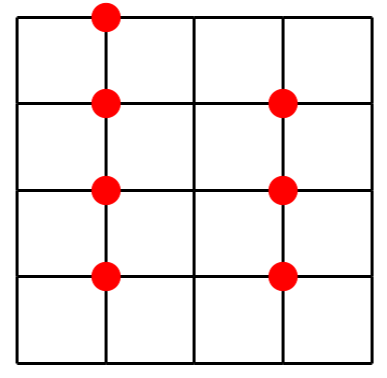
\includegraphics[scale=0.3]{figures/graph_exmp.png}
    \caption{Example of a $5 \times 5$ grid graph with obstacles (in \textcolor{red}{red})}
    \label{fig:graph_exmp}
\end{figure}

Figure~\ref{fig:graph_exmp} shows one of the graphs artificially built for this project. This particular graph has $7$ obstacle nodes, drawn in red, and $18$ valid nodes (not drawn). Every graph considered in this project is unweighted, although this is not a mandatory assumption, since it only needs a re-definition on the exploration budget $T$ to incorporate the weights of the edges. \\
The aim of the coverage process can be formalized as the following maximization problem:
\begin{equation}
    \max_{\{a_1, \dots, a_T\}} \sum_{n \in \mathcal{N}_v} \frac{c_T(n)}{|\mathcal{N}_v|}
\end{equation}
where $\{a_1, \dots, a_T\}$ is a sequence of $T$ actions and $\mathcal{N}_v$ is the set of all valid nodes, i.e. the nodes that can be visited. In this project every environment considered had at least $1$ obstacle node, hence $\mathcal{N}_v \subset \mathcal{N}$.

\subsection{Formalism}
A Reinforcement Learning (RL) agent interacts with an environment over time. At each time step $t$, the agent receives a state $s_t$ in a state space $\mathcal{S}$ and selects an action $a_t$ from an action space $\mathcal{A}$, following a policy $\gamma(s_t, a_t)$, which represents the agent’s behavior. The agent then receives from the environment a scalar reward $r_t$ and transitions to the next state $s_{t+1}$ according to the environment dynamics, through, respectively, a reward function $R(s_t,a_t)$ and a transition function $\varphi(s_{t+1}|s_t,a_t)$. \\
In this setting the state space coincides\footnote{In this case $\mathcal{S}$ is implemented as the graph configuration in addition to a minimum number of information, such as the number of visits for every valid nodes. This, however, do not drastically voids the simplification that $\mathcal{S} = \mathcal{N}_v$.} with the set of valid nodes $\mathcal{N}_v$, hence the state $s_t$ can be thought as the node $n_t$ visited at time step $t$. The action space, in a generic node $n$, is composed of at most $4$ actions: the agent can indeed move \textit{left}, \textit{up}, \textit{right} or \textit{down}.

\subsection{Reward}

The first (and most natural) reward function that has been considered was simply the normalized difference of visited nodes between the current time step and the previous one. 
\begin{equation}
    r_t = \frac{1}{|\mathcal{N}_v|} \Big [ \sum_{n \in \mathcal{N}_v} c_t(n) - c_{t-1}(n) \Big ] = \begin{cases}
    1/|\mathcal{N}_v| & \text{if a new node is visited} \\
    0 & \text{otherwise}
    \label{eq:rt1}
    \end{cases}
\end{equation}
This reward function (and a few variations of it considered) did not suit the training process, as it appeared unable to produce any improvement during the learning phase.\\
In the end the reward function that produced positive results, at least in the setting proposed, has this sparse definition:
\begin{equation}
    r_t = \begin{cases}
    -0.1 \cdot vis(n) & \text{if } n \in \mathcal{N}^*_t \\
    0.1 & \text{if } n \notin \mathcal{N}^*_t \\
    -0.5 & \text{if } n \notin \mathcal{N}_v
    \label{eq:rt2}
    \end{cases}
\end{equation}
where $\mathcal{N}^*_t \subseteq N_v$ is the set of visited nodes up to time step $t$ and $vis : \mathcal{N} \to \mathbb{N}$ is a function that counts the number of time that a node $n$ has been visited. This reward function punishes the agent for visiting the same state again, with a penalty proportional to the number of visits, and gives a positive reward when the agent visits a new state. Finally, when the agent tries to reach an obstacle or tries to exit the map a negative feedback of $-0.5$ is given.

\section{Implementation}
Deep Reinforcement Learning (DRL) has been successfully applied to a number of problems~\cite{deeprl}, thanks to the recent
advances in GPU computing. In this project DRL, and in particular the Deep Q-Network~\cite{mnih2015humanlevel} algorithm (DQN), has been applied in order to experiment with a simple yet non-trivial exploration task. Since the environments considered in this application are graphs, the DRL agent has been equipped with two Graph Neural Networks\cite{gnn} (GNN) in order to internally encode and represent the graph-structured data.\\
The Q-network\footnote{Following the nomenclature in~\cite{mnih2015humanlevel} the \textit{Q-network} is the one responsible for approximating the action-value function, while the \textit{target} network is the one used for estimating its value.} GNN here is used to approximate the optimal action-value function $Q^o(s, a)$, defined as
\begin{equation}
    Q^o(s, a) = \max_{\gamma} \mathbb{E} \Big [r_t + \alpha r_{t+1} + \alpha^2 r_{t+2} + \dots | s_t = s, a_t = a, \gamma \Big ]
\end{equation}
which is the maximum sum of rewards $r_t$ at each time-step $t$, discounted by $\alpha \in [0,1]$, achievable by a policy $\gamma$ when the agent is in the state $s$ and takes an action $a$. Another identically-structured GNN, namely the target network, is used to estimate the value of the action proposed by the online network.
Naming $s = s_t$, $s^{\prime} = s_{t+1}$, $a^{\prime} = a_{t+1}$ and $r = r_t$ we can define the \textit{experience} as $e = \{s, a, r, s^{\prime}\}$, that, at each time-step $t$, is stored in a data-set $D_t : D_t = \{e_1, \dots, e_t\}$. In order to reduce the correlation between the samples drawn from the data-set during the learning phase, a mini-batch $B$ is uniformly sampled from $D$ and Stochastic Gradient Descent (SGD) (in our case Adam) is applied on it. The target network then calculates the target value $r + \alpha \max_{a^{\prime}} Q(s^{\prime}, a^{\prime})$ and the Q-learning update is operated through the use of the Mean Squared Error loss function:

\begin{equation}
    L(\theta) = \mathbb{E}_{(s,a,r,s^{\prime}) \sim \mathcal{U}(D)} \Big [ \big ( r + \alpha \max_{a^{\prime}} Q(s^{\prime}, a^{\prime}; \theta^{-}) - Q(s, a; \theta) \big )^2 \Big ]
\end{equation}

where an explicit reference has been made on the different weights of the two networks: $\theta$ is used to parametrize the Q-network while $\theta^{\prime}$ is used for the target network. Finally, at the end of every learning step, a soft weights update is operated using the following formula
\begin{equation}
    \theta^{\prime} \leftarrow \beta \theta + (1-\beta)\theta^{\prime}
\end{equation}

\subsection{Model}
The GNN used in this project is a sequential model constructed over the Gated Graph Sequence Networks, a model proposed in~\cite{li2015gated} that augments the GNN structure with a Recurrent Neural Network. The GNN used in this project implements a mapping $G: (\mathcal{G}, \mathbb{R}^{\nu \times f}) \to [0,1]^4$, taking as inputs both the graph $\mathcal{G}$ and a $\nu \times f$ feature matrix. This function then outputs a $4$D real-valued vector, which contains the approximations for the optimal actions' value.\\
In our case $\nu = |\mathcal{N}| = 5^2 = 25$ and $f=7$, indicating the fact that every node has $7$ features. These $7$ features for the $i$-th node at time $t$ are indicated by $\mu_i^{(t)} = [x_i, y_i, o_i, vis_i^{(t)}, w, n_i^v, b^{(t)}]$ and are defined as
\begin{enumerate}
    \item $x_i \in \mathbb{R}$: The $x$ coordinate of the node.
    \item $y_i \in \mathbb{R}$: The $y$ coordinate of the node.
    \item $o_i \in \{0, 1\}$: A boolean flags indicating if the node is an obstacle.
    \item $vis_i^t \in \mathbb{N}$: The visit count for the node.
    \item $w \in \{0, 1\}$: A boolean flag indicating if the node is part of the perimetral wall.
    \item $n_i^v \in \mathbb{N}$: The number of node's neighbors that have not been visited yet.
    \item $b^t \in \{0, 1\}$: A boolean flag indicating if the agent is currently visiting the node.
\end{enumerate}
Features $4, 6$ and $7$ are time-dependant, hence the feature matrix $\mathcal{F}^{(t)} = [\mu_1^{(t)}, \dots, \mu_\nu^{(t)}]^\intercal$ evolves through time, reflecting the actions taken by the agent. \\
The sequential model built for this application is schematized in Table~\ref{tab:net}, where the \texttt{GateGNN} layer refers to the operator defined in~\cite{li2015gated}, \texttt{BatchNorm} to a batch normalization layer and \texttt{Linear} to a fully connected MLP. The dropout operation was carried with a drop probability of $p = 0.5$ while \texttt{GlobalPool} operator simply sums the rows of the input matrix on which it acts on. The ELU~\cite{clevert2015fast} function has been used as the activation function.  

\begin{table}[h]
\begin{tabular}{cllll}
\toprule
\# & Layer            & Input     & Ouput     & Params \\
\midrule
1      & \texttt{GatedGNN}$(7,4)$    & $(25, 7)$   & $(25, 7)$   & $532$             \\
2      & \texttt{BatchNorm}$(7)$     & $(25, 7)$   & $(25, 7)$   & $14$              \\
3      & \texttt{GatedGNN}$(64,4)$   & $(25, 7)$   & $(25, 64)$  & $26598$           \\
4      & \texttt{BatchNorm}$(64)$    & $(25, 64)$  & $(25, 64)$  & $128$             \\
5      & \texttt{GatedGNN}$(128,4)$  & $(25, 64)$  & $(25, 128)$ & $164608$          \\
6      & \texttt{GlobalPool}         & $(25, 128)$ & $(1, 128)$  & $-$               \\
7      & \texttt{Linear}$(128, 256)$ & $(1, 128)$  & $(1, 256)$  & $33024$           \\
8      & \texttt{Dropout}            & $(1, 256)$  & $(1, 256)$  & $-$               \\
9      & \texttt{Linear}$(256, 4)$   & $(1,256)$   & $(1,4)$     & $1028$            \\
\bottomrule
\end{tabular}
\caption{Network structure}
\label{tab:net}
\end{table}

The \href{https://pytorch-geometric.readthedocs.io/en/latest/modules/nn.html#torch_geometric.nn.conv.GatedGraphConv}{\texttt{GatedGNN}} implements a message passing operation that uses a RNN (a GRU~\cite{gru}) that can be roughly schematized as this couple of equations
\begin{equation}
    \begin{cases}
    m_i^{(l+1)} = \sum_{j \in \mathcal{N}_i} \Theta \cdot h_j^{(l)} \\
    h_i^{(l+1)} = \text{GRU}(m_i^{(l+1)}, h_i^{(l)})
    \label{eq:loop}
    \end{cases}
\end{equation}
that are iterated from $l=0$ up to $l=L-1$, where $L$ the number of the sequence length (in our case $L=4$, being this the second argument of the \texttt{GatedGNN} layer). The matrix $\Theta$ is the weight matrix and $\mathcal{N}_i$ is the set of neighbors for the $i$-th node. \\
The whole implementation was made using \href{https://pytorch.org/}{\texttt{PyTorch}}~\cite{paszke2017automatic} and the Neural Network has been built with \href{https://pytorch-geometric.readthedocs.io/en/latest/}{\texttt{PyTorch-Geometric}}~\cite{Fey/Lenssen/2019}
\subsection{Experiments and Results}
The general training scheme is shown in Algorithm \ref{alg:algo}, and it is substantially the same as the one proposed in~\cite{mnih2015humanlevel} and briefly explained above, which makes use of the experience replay mechanism. Experiments have been made also using the Double Deep Q-Network (DDQN) algorithm~\cite{drldql}, but the best results were reached with DQN. 

\begin{algorithm}
\caption{: GraphDRL}\label{euclid}
\begin{algorithmic}[1]
\State Initialize experience replay memory $\mathbf{M}$
\State Initialize environment $\mathcal{G}$
\State Initialize networks weights $\theta, \theta^{\prime}$
\For {episode $e = 1 \dots E$}
\State Reset $\mathcal{G}$ and construct initial state $s_0$
\For {step $t = 1 \dots T$}
\State Select action $a_t$ following an $\epsilon$-strategy
\State Execute action $a_t$, receive reward $r_t$ and move to state $s_{t+1}$
\State Store transition $(s_t, a_t, r_t, s_{t+1})$ in $\mathbf{M}$
\State Sample a random minibatch $B$ from $\mathbf{M}$
\State Update $\theta$ by SGD for $B$%: $\theta \leftarrow \theta - l\sum_{b \in B} \frac{d}{d\theta}Q(s,a; \theta) \big ( \big )$
\State Soft update $\theta^{\prime}$
\EndFor
\EndFor
\State Return $\theta$
\end{algorithmic}
\label{alg:algo}
\end{algorithm}

A total number of $10$ environments has been used: $1$ for training the agent and the other $9$ for testing. These 10 simple graphs have been created artificially for this project. All the experiments have been carried out in the \href{https://colab.research.google.com/}{\texttt{Google Colab}} environment, where a Tesla K80 GPU was available.\\
Several runs with different hyperparameters gave comparable results, but, due to the limited (yet fairly powerful) amount of resources available, an hyperparameters optimization procedure could not be accomplished. The results shown below may not be the best that can be reached by this model.\\
The hyperparameters used are $|B| = 32$, $\beta = 10^{-3}$, $\alpha = 0.99$ and a learning rate of $10^{-3}$. The total number of episodes is $E = 10^4$ with $T = 25$ for each episode. In Figure~\ref{fig:train} are shown a few metrics logged by \href{https://www.tensorflow.org/tensorboard/}{\texttt{Tensorboard}}. These metrics are, respectively, the $\epsilon$-decaying policy (which is exponential) (\ref{fig7:a}), the loss function (\ref{fig7:b}), the number of nodes visited in an episode (\ref{fig7:c}) and the reward gained in an episode. These metrics were logged once in 10 episodes and the agent starting node has been randomized at the beginning of every step.

\begin{figure}[ht] 
  \begin{subfigure}[b]{0.5\linewidth}
    \centering
    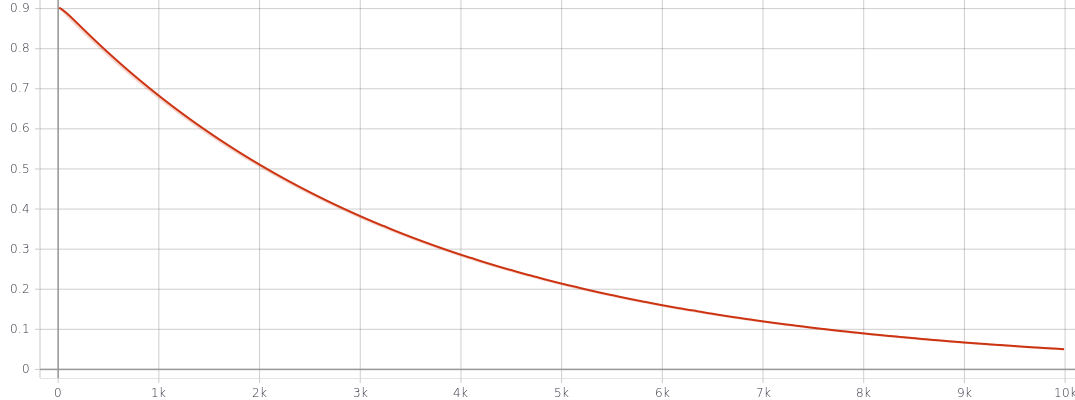
\includegraphics[width=0.75\linewidth]{figures/eps.png} 
    \caption{$\epsilon$-decay function} 
    \label{fig7:a} 
    \vspace{4ex}
  \end{subfigure}%% 
  \begin{subfigure}[b]{0.5\linewidth}
    \centering
    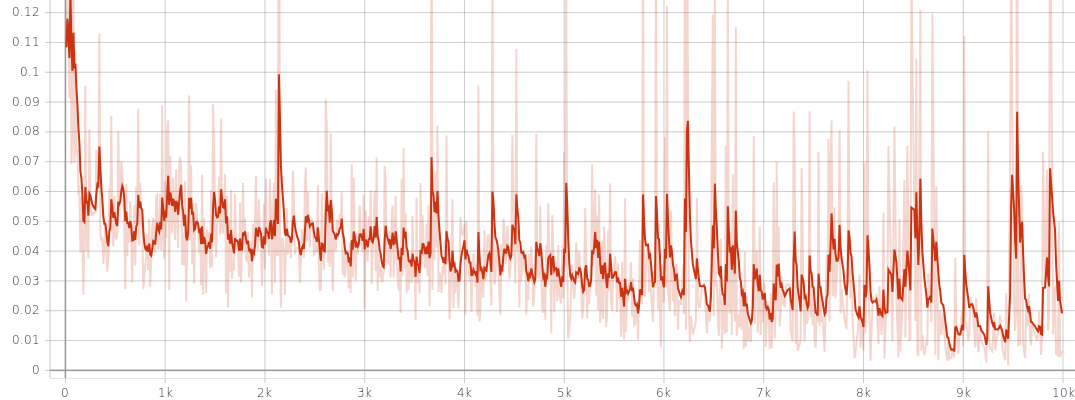
\includegraphics[width=0.75\linewidth]{figures/loss.png} 
    \caption{Loss} 
    \label{fig7:b} 
    \vspace{4ex}
  \end{subfigure} 
  \begin{subfigure}[b]{0.5\linewidth}
    \centering
    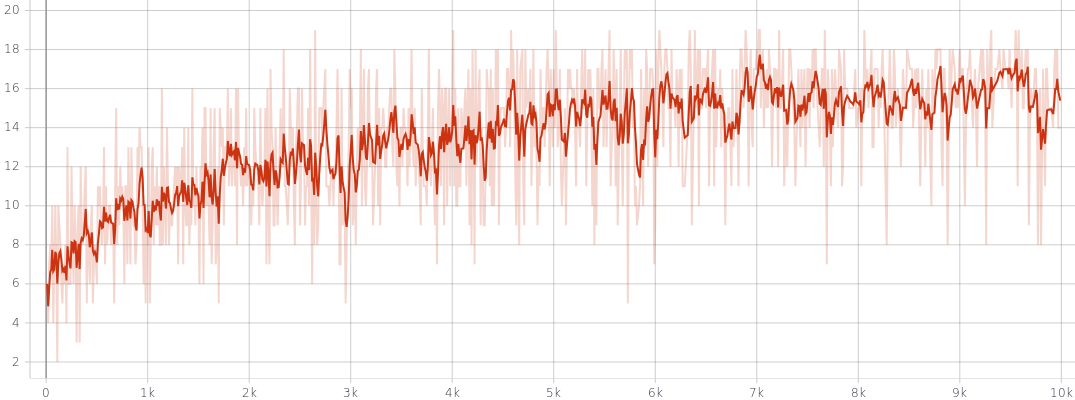
\includegraphics[width=0.75\linewidth]{figures/nodes.png} 
    \caption{Nodes visited} 
    \label{fig7:c} 
  \end{subfigure}%%
  \begin{subfigure}[b]{0.5\linewidth}
    \centering
    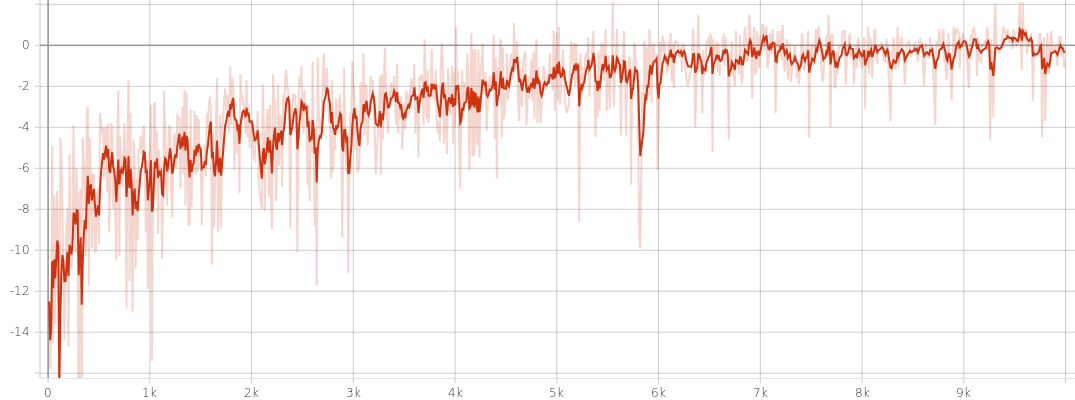
\includegraphics[width=0.75\linewidth]{figures/reward.png} 
    \caption{Reward} 
    \label{fig7:d} 
  \end{subfigure} 
  \caption{A few metrics from the training phase}
  \label{fig7} 
 \label{fig:train}
\end{figure}

\subsection{Testing}

The testing phase has been executed in a similar manner. After the environment initialization the agent started exploring the graph, following exclusively the action proposed by the Q-network. This was done for 30 episodes of 25 steps each, for every environment in the test-set. At the end of every episode percentage of valid nodes visited by the agent has been registered. The results for these tests can be seen in Table~\ref{tab:res}, which are expressed in terms of mean ($\mu$), standard deviation ($\sigma$) and \textit{Best Run}. The latter is the best percentage (highest number of valid nodes visited) during an episode, by the agent.

\begin{table}[h]
\begin{tabular}{cccc}
\toprule
\textit{Env} & $\mu$ & $\sigma$  & \textit{Best Run} \\
\midrule
a$^*$   & 89.8 & 8.3  & 100      \\
b   & 61.9 & \textbf{25.6} & 88.9     \\
c   & 78.5 & 10.7 & 94.4     \\
d   & \textit{55.2} & 20.7 & 88.9     \\
e   & 74.0 & 9.5  & 89.5     \\
f   & 62.6 & 18.0 & 83.3     \\
g   & 71.4 & 19.1 & 88.2     \\
h   & 63.5 & 11.1 & \textit{81.0}     \\
i   & 56.0 & 23.9 & 85.0     \\
j   & \textbf{82.1} & \textit{9.2}  & \textbf{95.5}    \\
\bottomrule
\end{tabular}
\caption{Mean and standard deviation wrt the normalized node coverage, for every environment, during 30 episodes of 25 steps each. The graph marked with the asterisk* is the one on which the agent has been trained. The \textbf{maximum} and \textit{minimum} for every column are marked in bold and italics, respectively.}
\label{tab:res}
\end{table}

\begin{figure}[ht] 
  \begin{subfigure}[b]{0.2\linewidth}
    \centering
    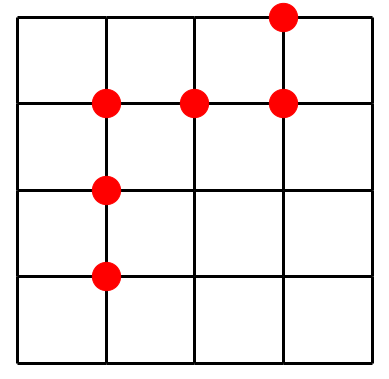
\includegraphics[width=0.75\linewidth]{figures/maze_5x5_0.png} 
    \caption{} 
    \vspace{4ex}
  \end{subfigure}%% 
  \begin{subfigure}[b]{0.2\linewidth}
    \centering
    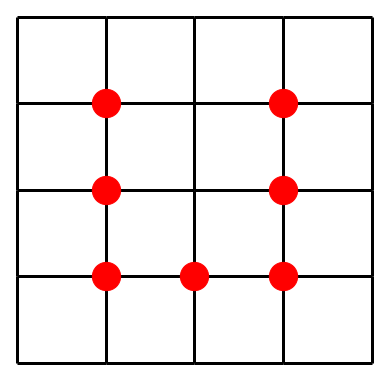
\includegraphics[width=0.75\linewidth]{figures/maze_5x5_1.png} 
    \caption{} 
    \vspace{4ex}
  \end{subfigure}%%
    \begin{subfigure}[b]{0.2\linewidth}
    \centering
    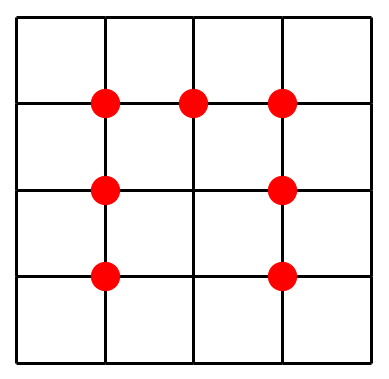
\includegraphics[width=0.75\linewidth]{figures/maze_5x5_2.png} 
    \caption{} 
    \vspace{4ex}
  \end{subfigure}%% 
    \begin{subfigure}[b]{0.2\linewidth}
    \centering
    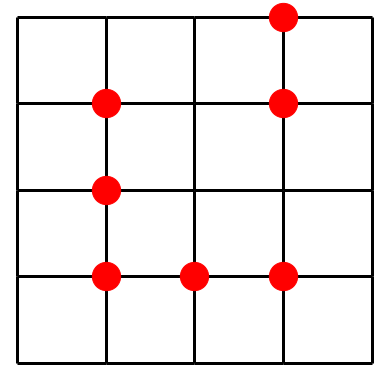
\includegraphics[width=0.75\linewidth]{figures/maze_5x5_3.png} 
    \caption{} 
    \vspace{4ex}
  \end{subfigure}%% 
    \begin{subfigure}[b]{0.2\linewidth}
    \centering
    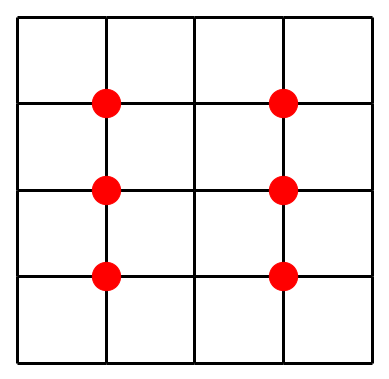
\includegraphics[width=0.75\linewidth]{figures/maze_5x5_4.png} 
    \caption{} 
    \vspace{4ex}
  \end{subfigure}
    \begin{subfigure}[b]{0.2\linewidth}
    \centering
    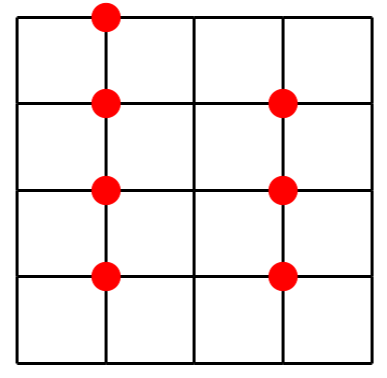
\includegraphics[width=0.75\linewidth]{figures/graph_exmp.png} 
    \caption{} 
    \vspace{4ex}
  \end{subfigure}%% 
  \begin{subfigure}[b]{0.2\linewidth}
    \centering
    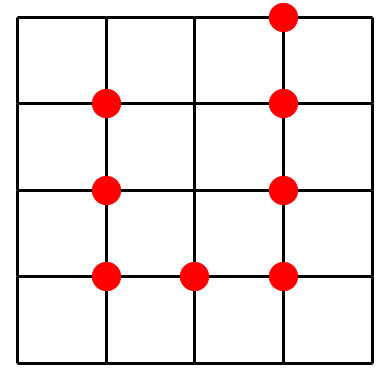
\includegraphics[width=0.75\linewidth]{figures/maze_5x5_6.png} 
    \caption{} 
    \vspace{4ex}
  \end{subfigure}%%
    \begin{subfigure}[b]{0.2\linewidth}
    \centering
    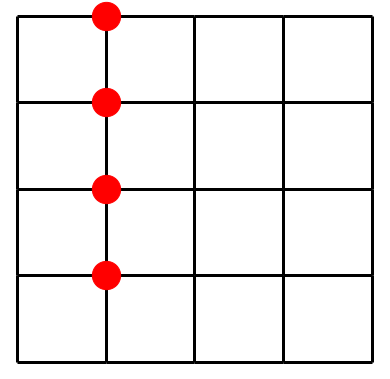
\includegraphics[width=0.75\linewidth]{figures/maze_5x5_7.png} 
    \caption{} 
    \vspace{4ex}
  \end{subfigure}%% 
    \begin{subfigure}[b]{0.2\linewidth}
    \centering
    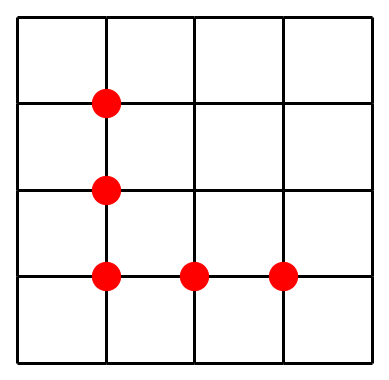
\includegraphics[width=0.75\linewidth]{figures/maze_5x5_8.png} 
    \caption{} 
    \vspace{4ex}
  \end{subfigure}%% 
    \begin{subfigure}[b]{0.2\linewidth}
    \centering
    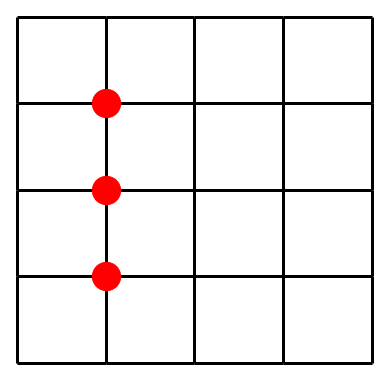
\includegraphics[width=0.75\linewidth]{figures/maze_5x5_9.png} 
    \caption{}
    \vspace{4ex}
  \end{subfigure}
\end{figure}

Apart from the training graph (a), we can see from Table~\ref{tab:res} that the best results were achieved on graph (j). This is clearly the simplest graph in the set, hence the mean coverage is quite high (82.1\%) and the standard deviation fairly low compared to the others. This graph is almost identical to (h), except for the node at the (0,1) position. The performances on this graph were significantly worse and this performance drop might be related to the node (or edge) connectivity.\\

Despite the simple structure of the environments, the policy obtained with this method seems adequate for being at least a simple baseline for comparisons with more complex algorithms. Deep Reinforcement Learning with Graph Neural Networks (and Geometric Deep Learning in general) is at the first stages of development and so this project can also be a starting point for future and more evolved (and theoretically grounded) experiments.

\newpage
\noindent\rule[0.25\baselineskip]{\textwidth}{1pt}

\bibliography{mybib}{}
\bibliographystyle{ieeetr}



\end{document}